\chapter{Estado del Arte\label{sec:estado_del_arte}}

En este capítulo se estudia más detalladamente el problema que pretende resolver el proyecto y las características del entorno.


%--Enfermedades
\section{Enfermedades neurológicas}
\label{sec:dolencias2}

Las enfermedades neurológicas son muy frecuentes en España. Los servicios de neurología atienden a más de 2.2 millones de pacientes al año. Además, 7.5 millones de personas sufren algún tipo de enfermedad neurológica (un 16\% de la población española). 

Se conocen dos tipos de accidentes cerebrovasculares (ACV) según la causa \cite{tipoIctus}:
\begin{itemize}
	\item Hemorragia cerebral: suceden  a causa de la rotura de una vaso sanguíneo.
	\item Isquemia cerebral: consecuencia de una obstrucción de una arteria por la presencia de un coágulo de sangre. En muchas ocasiones se origina en el corazón y se desplaza hasta el cerebro, dónde interrumpe el flujo sanguíneo.
\end{itemize}

Sea cual sea la causa del ictus, el daño cerebral adquirido puede ser irreversible. Las secuelas posteriores pueden repercutir considerablemente en la calidad de vida del afectado.

Cuando se sufre un accidente cerebrovascular es recomendable recibir atención neurológica temprana, preferentemente durante la primera hora. Cuanto más tiempo se tarde en recibir atención por un especialista, peores serán las consecuencias del accidente y más complicada la recuperación.

Este tipo de enfermedades habitualmente son atendidas por los servicios de urgencias, debido a que surge de manera fortuita y sus efectos instantáneos son de gran magnitud. De los 26 millones de urgencias hospitalarias que se atienden al año en España, el 14\% son neurológicas y en su gran mayoría son consideradas de nivel I-III (riesgo vital-riesgo potencial). Asimismo, neurología es la segunda especialidad más requerida en los servicios de urgencias.

Existe una medida denominada DALY (años de vida ajustados por discapacidad) que estima el número de años perdidos por causa de una enfermedad, discapacidad o muerte prematura. Según la cual sitúa el ICTUS como la más influyente (con el 55\% entre las demás) de entre dolencias como: alzheimer (12\%), migraña (8.3\%), epilepsia (7.9\%), parkinson, esclerosis múltiple, meningitis y otros. Este hecho señala la importancia de conseguir poner remedio a esta situación, consiguiendo que el ictus no sea tan significativo en este tipo de medidas.

El ictus tiende a prevalecer más en el enfermo cuanto mayor es su edad. Es decir, cuanto mayor edad tiene la persona afectada, más difícil es la recuperación de este. \cite{pentienII}

\subsection{Secuelas}
\label{sec:secuelas}

Los afectados por esta enfermedad padecen una serie de secuelas físicas y sensoriales de difernetes tipos que se citan a continuación:

\begin{itemize}[label=$ \rhd $]
	\item \underline{Alteraciones de tono muscular:} Espasticidad, hipertonía, hipotomía, distonía, pérdida de simetría, movimiento enlentecido, movimiento en bloque, alteraciones en la coordinación, luxaciones/subluxaciones y edemas.
 
	\item \underline{Paresia o parálisis:} Monoplejia, hemiplegia/hemiparesia, paraplegia, tetraplejia/tetraparesia.
	\item \underline{Pérdida de las sensaciones táctiles y propioceptivas}
	\item \underline{Fatiga}
	\item \underline{Alteraciones de equilibrio y coordinación}
\end{itemize}

Cuando una persona sufre una enfermedad neurológica son varios los aspectos de sus vida en los que necesita ayuda para volver a llevar una vida autonoma:
	\begin{itemize}
 		\item Cuidado médico para revisar el estado de su salud personal
 		\item Logoterapia y terapia ocupacional para mejorar la comunicación con el entrono 
 		\item Grupos de apoyo y soporte familiar para cubrir las necesidades psicosociales
		\item Control en la mejora de la condición física del paciente para conseguir autonomía en la vida diaria a través de rehabilitación a largo plazo. Actividad que es guiada gracias a los profesionales fisioterapeutas.
		
	
	\end{itemize}


\subsection{Rehabilitación}
\label{sec:neuronal2}

Tras el alta hospitalaria el paciente requiere un largo periodo de rehabilitación para poder realizar tareas cotidianas como subir escaleras, vestirse, ir al baño, asearse, alimentarse y pasear. \cite{secuelasIctus}

De entre estas seis actividades de la vida diaria, para poder realizar algunas de ellas es necesario tener el control del movimiento de las manos. Se utilizan las manos para muchísimas más tareas de la vida cotidiana, pero en este tipo de pacientes se procura primero recuperar la capacidad mínima y así se puedan valer por si mismos en las tareas más básicas y vitales.

Para poder lograr minimizar los impedimentos físicos que experimentan estos pacientes la rehabilitación juega un papel fundamental. Esto ayuda además a la recuperación de la vida social de estas personas. 


\section{Rehabilitación de las manos}
\label{sec:fuindamentos2}

Las manos son una parte del cuerpo humano con una funcionalidad muy importante en el día a día de las personas. En la figura \ref{fig:anatomiaMano} se observan las falanges que componen las manos. 

\begin{figure}[H]
	\centering
	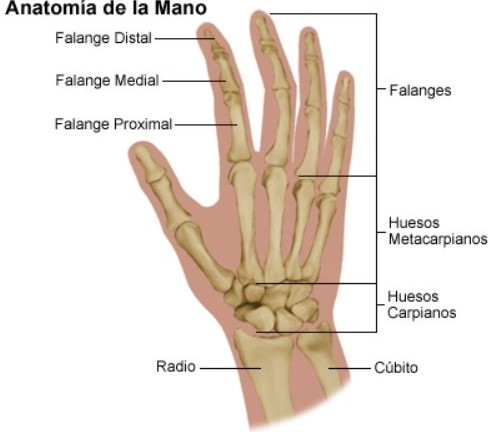
\includegraphics[width=0.5\textwidth]{./img/anatomiaMano}
	\caption{Anatomía de las manos.  \cite{imgAnatomiaMano}}
	\label{fig:anatomiaMano}
\end{figure} 

Cuando un persona ha sufrido un ictus en muchas ocasiones pierde la movilidad total o parcial de la mano. Es importante comprender que en este tipo de afecciones el problema no se inicia en un defecto físico de la mano, sino en los músculos. A consecuencia del ACV estos han deshabilitado la capacidad de enviar pulsos eléctricos a esta extremidad. Entendidos como las señales que envía el cerebro a la mano para que esta se mueva. Lo que se pretende recuperar mediante rehabilitación es tanto la comunicación entre el cerebro y el músculo como la capacidad física de movimiento, ya que cuanto más tiempo pasa un músculo sin moverse, este va perdiendo habilidad para moverse. Por ello, es muy importante trabajar el movimiento de los músculos aunque estos no sean capaces de moverse por si mismos.


Existen muchos tipos de técnicas de tratamiento para fomentar el trabajo de las funcionalidades de las extremidades superiores: técnicas manuales, entrenamiento motor orientado a tareas, ferulaje, vendaje neuromuscular, electroestimulación funcional, %Se estimulan los músculos mediante impulsos electricos para que este se mueva.
mirror therapy, %Se pone un espejo entre las dos extremidades, reflejando la mano que tiene capacidad de movimiento. El ejercicio consiste en mover la mano sana para estimular mediante el espejo a que el cerebro muevo la otra.
realidad virtual y rehabilitación robótica.


El objetivo es recuperar la máxima funcionalidad de las extremidades superiores, lo que resulta en mejorar el rango de movimiento activo y parámetros como fuerza, coordinación, sensibilidad y destreza manipulativa.

Durante los ejercicios de rehabilitación es necesario realizar muchos tipos de movimientos. En la figura \ref{fig:movManos} se representan los movimientos de las manos. %Estos movimientos debería de ser capaz de realizar un prototipo que tenga por función de medir el movimiento de las manos adherido a estas:

\begin{figure}[H]
	\centering
	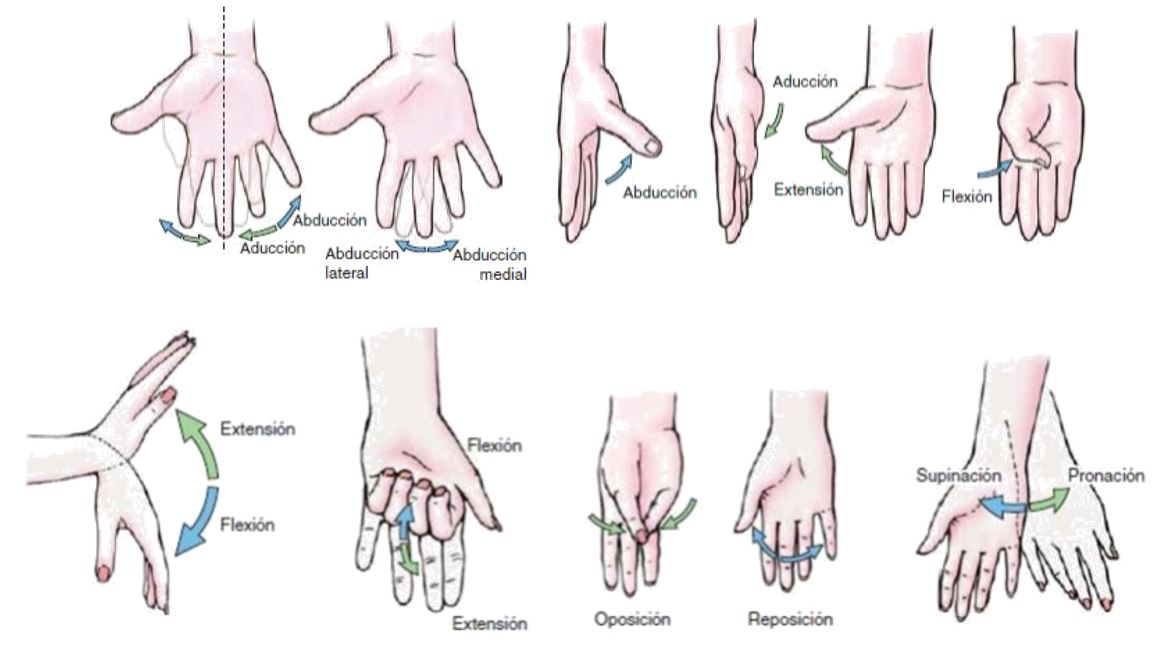
\includegraphics[width=0.85\textwidth]{./img/ejerciciosRehManp}
	\caption{Movimientos de las manos \cite{movimientoMano}} 
	\label{fig:movManos}
\end{figure}


\section{Guantes sensorizados}
\label{sec:captura2}

Gracias a la tendencia innovadora en la sociedad actual, sucede la inserción de nuevos desarrollos tecnológicos en el marco de la rehabilitiación. Los avances en la tecnología han permitido un gran desarrollo en los dispositivos de análisis del movimiento de las manos.

Se han llevado a cabo investigaciones sobre guantes sensorizados a base de fibra óptica para aplicaciones biomecatrónicas y clínicas, que permiten el análisis de la flexo-extensión de las articulaciones interfalangiales proximales y metacarpofalangiales de los dedos índice, corazón, anular y meñique, al igual que de la articulación interfalangial y metacarpofalangial del dedo pulgar. Esto es, un análisis limitado a 10 grados de libertad (GDL), cuando la mano humana se suele modelar con 21 GDL. Sin embargo, no se ha podido encontrar ningún producto comercial que cumpla este propósito mediante esta tecnología.

Existen varios productos en el mercado que utilizando sensores de flexión son capaces de medir los movimientos de los dedos y así realizar diagnósticos centrados en la capacidad flexo-extensora del paciente. Ejemplo de ello son los dos guantes comercializados por CyverGloveSystems (ver figura \ref{fig:CGS}) \cite{CGS}

\begin{figure}[H]
	\centering
	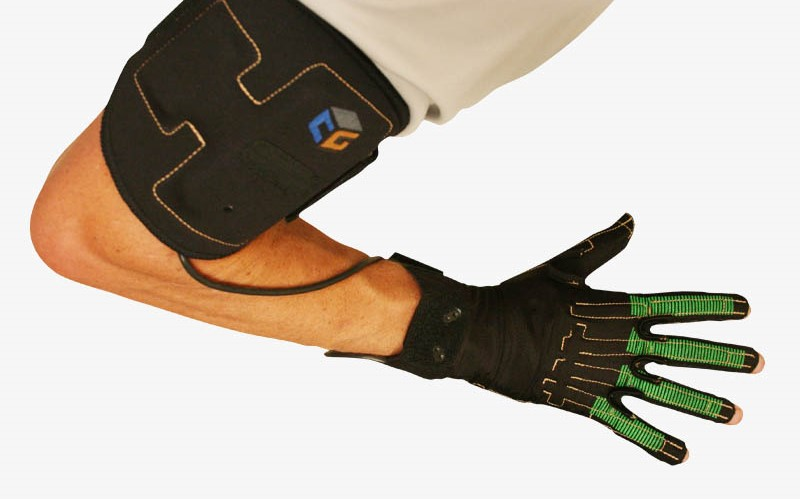
\includegraphics[width=0.5\textwidth]{./img/cgs}
	\caption{Modelo CyberGlove III de CyverGloveSystems. }
	\label{fig:CGS}
\end{figure} 

Existen productos en el mercado con otras tecnologías para medir la capacidad de movimiento de la mano. En la figura \ref{fig:rapael} se muestra Rapael, un guante que combina sersores de flexión y sensores inerciales o IMUs (Inertial Measurement Units). Estos últimos son muy versátiles en este tipo des escenarios ya que ofrecen una monitorización precisa de diversos parámetros, como la aceleración o la velocidad angular, además de ser ligeros y por tanto más fáciles de adaptar a un guante.

Además, Rapael se comercializa para medir la capacidad de movimiento de las manos de personas que han sufrido un accidente cerebrovascular. Un aspecto muy positivo de este guante es que es capaz de adaptarse a cualquier tipo de mano gracias a su diseño. También cuenta con una aplicación para tablet que monitoriza los ejercicios.

\begin{figure}[H]
	\centering
	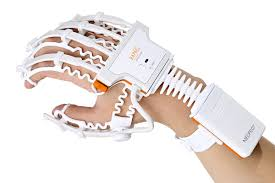
\includegraphics[width=0.5\textwidth]{./img/rapael}
	\caption{Modelo de guante Rapael }
	\label{fig:rapael}
\end{figure} 

 
Por otra parte, también es importante destacar los avances en técnicas de procesado de señal como algoritmos de reconstrucción, transformadas tiempo-frecuencia, análisis de componentes principales y técnicas de machine learning entre otras para el análisis de la información, la clasificación y el reconocimiento de patrones. Gracias a estas técnicas,  los softwares desarrollados en algunos de estos proyectos, a parte del propio guante, no sólo orientar a los pacientes y terapeutas en la rehabilitación. Tambien proporcionan una referencia de los movimientos a los que se someterán los sensores, lo cual permite optimizar el análisis de la de información.


%Para mejorar el proceso de rehabilitación resulta imprescindible avaluar el avance de las sesiones. Actualmente se utilizan mecanismos de medida que no resultan precisos (ver figura \ref{fig:medidaAnticuada}). Los datos obtenidos de estas mediciones no son lo suficientemente fiables como para que pueda cuantificarse realmente el avance de la condición del paciente.

%La solución a este cuestión es un sistema de medida capaz de realizar una valoración objetiva de la evolución de los pacientes. Lo cual permitiría al personal rehabilitador diseñar sesiones de rehabilitación más específicos para cada paciente y tener un mejor conocimiento d la repercusión de los ejercicios de rehabilitación en los pacientes. Mejorando además las prescripciones realizadas. 

%Este tipo de dispositivo se debe conseguir mediante el empleo de nuevas tecnologías incipientes. Es un buen momento para innovar en este ámbito ya que en estos últimos años se ha detectado un incremento de desarrollo tecnológico en el ámbito médico debido a las mejoras del servicio que ello conlleva. Igualmente sucede en el caso de tratamientos médicos para pacientes de ACV, es conveniente invertir en ello, ya que se ampliaría y mejoraría la modo en el que se aborda el tratamiento de la enfermedad a la larga. 

%E tipo de tecnología que se propone en este trabajo se enfoca a pacientes con ictus, pero igualmente podría servir en otros escenarios.

%\begin{figure}[H]
%	\centering
%	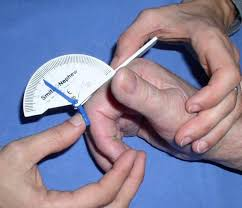
\includegraphics[width=0.4\textwidth]{./img/rehabAnti}
%	\caption{Mecanismo de medición de los ángulos de apertura de las articulaciones de la mano. } 
%	\label{fig:medidaAnticuada}
%\end{figure} 


%--TECNOLOGIAS MEDICIÓN
%Tecnologías para la medición del movimiento

%En la actualidad existen diferentes sistemas que permiten medir el movimiento. Entre ellos podemos enumerar:
%\begin{itemize}
%	\item {Cámaras}
%	\item {Fibras FBG}
%	\item {IMU}
%	\item {Sensores capacitivos}
%	\item {Sensores mioeléctricos}
%\end{itemize}

%Teniendo en cuenta la aplicación de este trabajo, y las deformaciones que tienen las manos a medir las dos tecnologías que mejor se adaptan al problema son las fibras FBG y los sensores inerciales.

%En este trabajo se estudian más en profundidad las fibras FBG y los sensores IMU. Para ello se han desarrollado un primer prototipo basado en las fibras de Bragg. Además, se ha propone un segundo prototipo basado en sensores inerciales. Notese que por prototipo se refiere a sistema hardware y software.


 